\newpage

\subsection{UC2 - Creazione di un grafico}
\label{subsec:uc2}

%TODO: Add correct image
\begin{figure}[h]
    \centering
    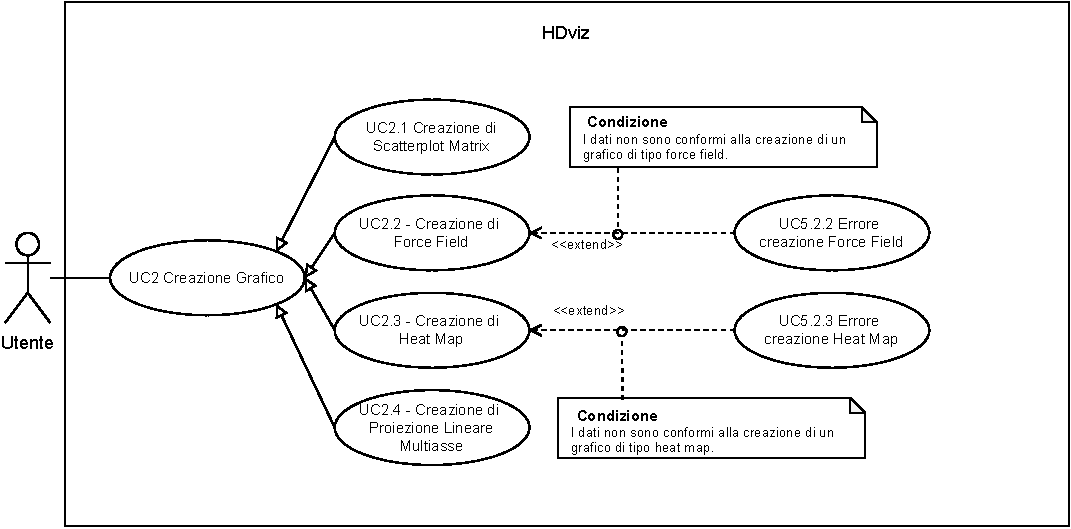
\includegraphics[width=0.8\textwidth]{componenti/casi-duso/diagrammi/UC2.pdf}
    \caption{Diagramma rappresentante UC2}
    \label{fig:UC2}
\end{figure}


\begin{itemize}
    \item \textbf{Descrizione}: L’utente vuole procedere con la fase di esplorazione
                                dati mediante la visualizzazione del dataset
                                attraverso uno dei diversi grafici proposti dall’applicativo
                                che ne costruisce uno e lo visualizza.
	
    \item \textbf{Attore primario}: Utente;
    
    \item \textbf{Precondizione}:   Nella sessione è stato importato un dataset e ogni 
                                    suo campo ha un metatag associato.

    \item \textbf{Postcondizione}:  Viene calcolato il grafico della tipologia scelta dai dati 
									dal dataset importato dotato di metatag validi e successivamente 
									visualizzato all'utente.

	\item \textbf{Scenario principale}:
		\begin{enumerate}
			\item L'utente seleziona l'opzione che desidera tra le tipologie di grafico.
			\item HDviz visualizza il grafico ottenuto dalla costruzione dei dati.
        \end{enumerate}

    \item \textbf{Generalizzazioni:}:  L'utente seleziona il grafico desiderato tra:

    \begin{enumerate}
        
        \item Grafico scatterplot matrix (UC2.1).
        \item Grafico force field (UC2.2).
        \item Grafico heat map (UC2.3).
        \item Grafico proiezione lineare multiasse (UC2.4).
        
	\end{enumerate}

\end{itemize}

% TODO: Make error for each selected graph type.
\subsubsection{UC2.1 Selezione di Scatterplot matrix}
\label{ssub:UC2.1}
\begin{itemize}

    \item \textbf{Attore primario}: Utente;

    \item \textbf{Precondizione}:   Un dataset è stato correttamente importato e ad ogni campo ha associato
                                    un metatag valido;

    \item \textbf{Postcondizione}:  Viene calcolato il grafico di tipo Scatterplot Matrix;

	\item \textbf{Scenario Principale}: HDviz costruisce un grafico Scatterplot matrix con il dataset 
										importato.
\end{itemize}


\subsubsection{UC2.2 Selezione di Force Field}
\label{ssub:UC2.2}
\begin{itemize}

    \item \textbf{Attore primario}: Utente;

    \item \textbf{Precondizione}:   Un dataset è stato correttamente importato e ad ogni campo ha associato
                                    un metatag valido;

    \item \textbf{Postcondizione}:  Viene calcolato il grafico di tipo Force Field;
	
	\item \textbf{Scenario Principale}: HDviz costruisce un grafico Force Field con il dataset importato.
	% Secondo me fa in scenario alternativo e in estensione solo lo UC a cui si riferisce. Pensaci
	% I pro apes fanno tutto in estensioni mentre i Qbeam fanno scenario alternativo e mettono in estensione solo UC riferimento
	\item \textbf{Estensioni}:
	\begin{enumerate}
		\item Se il dataset corrente non è compatibile con il grafico di tipo Force Field:
		\begin{enumerate}
			\item La costruzione del grafico fallisce.
			\item Viene visualizzato un messaggio di errore. (UC4.2.2)
		\end{enumerate}
	\end{enumerate}
\end{itemize}


\subsubsection{UC2.3 Selezione di Heat Map}
\label{ssub:UC2.3}
\begin{itemize}

    \item \textbf{Attore primario}: Utente;

	\item \textbf{Precondizione}:   Un dataset è stato correttamente importato e ad ogni campo 
									ha associato un metatag;

    \item \textbf{Postcondizione}:  Viene calcolato il grafico di tipo Heat map dal progetto corrente
	\item \textbf{Scenario Principale}: HDviz costruisce un grafico Heat Map con il dataset importato.
	% Secondo me fa in scenario alternativo e in estensione solo lo UC a cui si riferisce. Pensaci
	% I pro apes fanno tutto in estensioni mentre i Qbeam fanno scenario alternativo e mettono in estensione solo UC riferimento
	\item \textbf{Estensioni}:
	\begin{enumerate}
		\item Se il dataset corrente non è compatibile con il grafico di tipo Heat Map:
		\begin{enumerate}
			\item La costruzione del grafico fallisce.
			\item Viene visualizzato un messaggio di errore. (UC4.2.3)
		\end{enumerate}
	\end{enumerate}
\end{itemize}


\subsubsection{UC2.4 Selezione di Proiezione Lineare Multiasse}
\label{ssub:UC2.4}
\begin{itemize}

    \item \textbf{Attore primario}: Utente;

    \item \textbf{Precondizione}:   Un dataset è stato correttamente importato e ad ogni campo ha associato
                                    un metatag;

    \item \textbf{Postcondizione}:  Viene calcolato il grafico di tipo \emph{"Proiezione lineare multiasse"} dal progetto corrente

	\item \textbf{Scenario Principale}: HDviz costruisce un grafico Proiezione Lineare Multiasse con il dataset importato.
\end{itemize}

\subsubsection{UC2.5 Selezione di Distance Map}
\label{ssub:UC2.5}
\begin{itemize}
	\item \textbf{Descrizione}:			Viene selezionata la visualizzazione dei dati mediante graafico \emph{Distance Map}
	\item \textbf{Attore primario}:		Utente;
	\item \textbf{Precondizione}:		È stato importato correttamente un dataset (UC1 \refSec{sub:uc1})
	\item \textbf{Postcondizione}:		É stato selezionata la visualizzazione del grafico \emph{Distance Map} con i dati 
										precedentemente importati
	
	\item \textbf{Scenario Principale}: L'utente seleziona il grafico \emph{Distance Map} tra le opzioni proposte
\end{itemize}